\section{Introduction}\label{sec:introduction}

 Legged robots are among the most versatile robotic platforms available. As their natural counterpart, they show great flexibility and are particularly suited for applications where navigation through unstructured environments is required. 

The development of robots capable of fully exploiting the potential of legged morphology is, however, a non-trivial task, both in terms of design and control. There are several instances of robots that come close to achieving this.
% For instance, in~\cite{agile_bots::hawkes2022engineered} the authors employ the work multiplication principle to design and control a miniature robot capable of exceeding the jumping performance of any biological jumper. 
% A hybrid approach is employed by Ascento~\cite{agile_bots::klemm2019ascento}, which uses wheeled-locomotion for normal navigation and jumping motions generated with a multi-phase heuristic feed-forward controller to overcome challenging obstacles.
The autonomous quadruped ANYmal~\cite{agile_bots::hutter2016anymal} is, for instance, an example of a torque-controllable robot capable of robustly navigating through harsh industrial environments while performing complex locomotion tasks.

The potential of legged robots has begun to show its full realization only in recent years, culminating with the latest Boston Dynamics' ATLAS~\cite{agile_bots::atlas_gets_grip} performance, where human-like agile and complex jumping maneuvers were demonstrated on real hardware. The success of Boston Dynamics' approach shows how the convergence of both high-level hardware and carefully designed planning and control software is a critical requirement for future state-of-the-art robots. 
% ATLAS~\cite{agile_bots::atlas_gets_grip} platform provides a rare - if not unique - example of a high-payload yet extremely agile robot which, differently from our platform, is hydraulically powered.  
\begin{figure}[t]
    \centering
    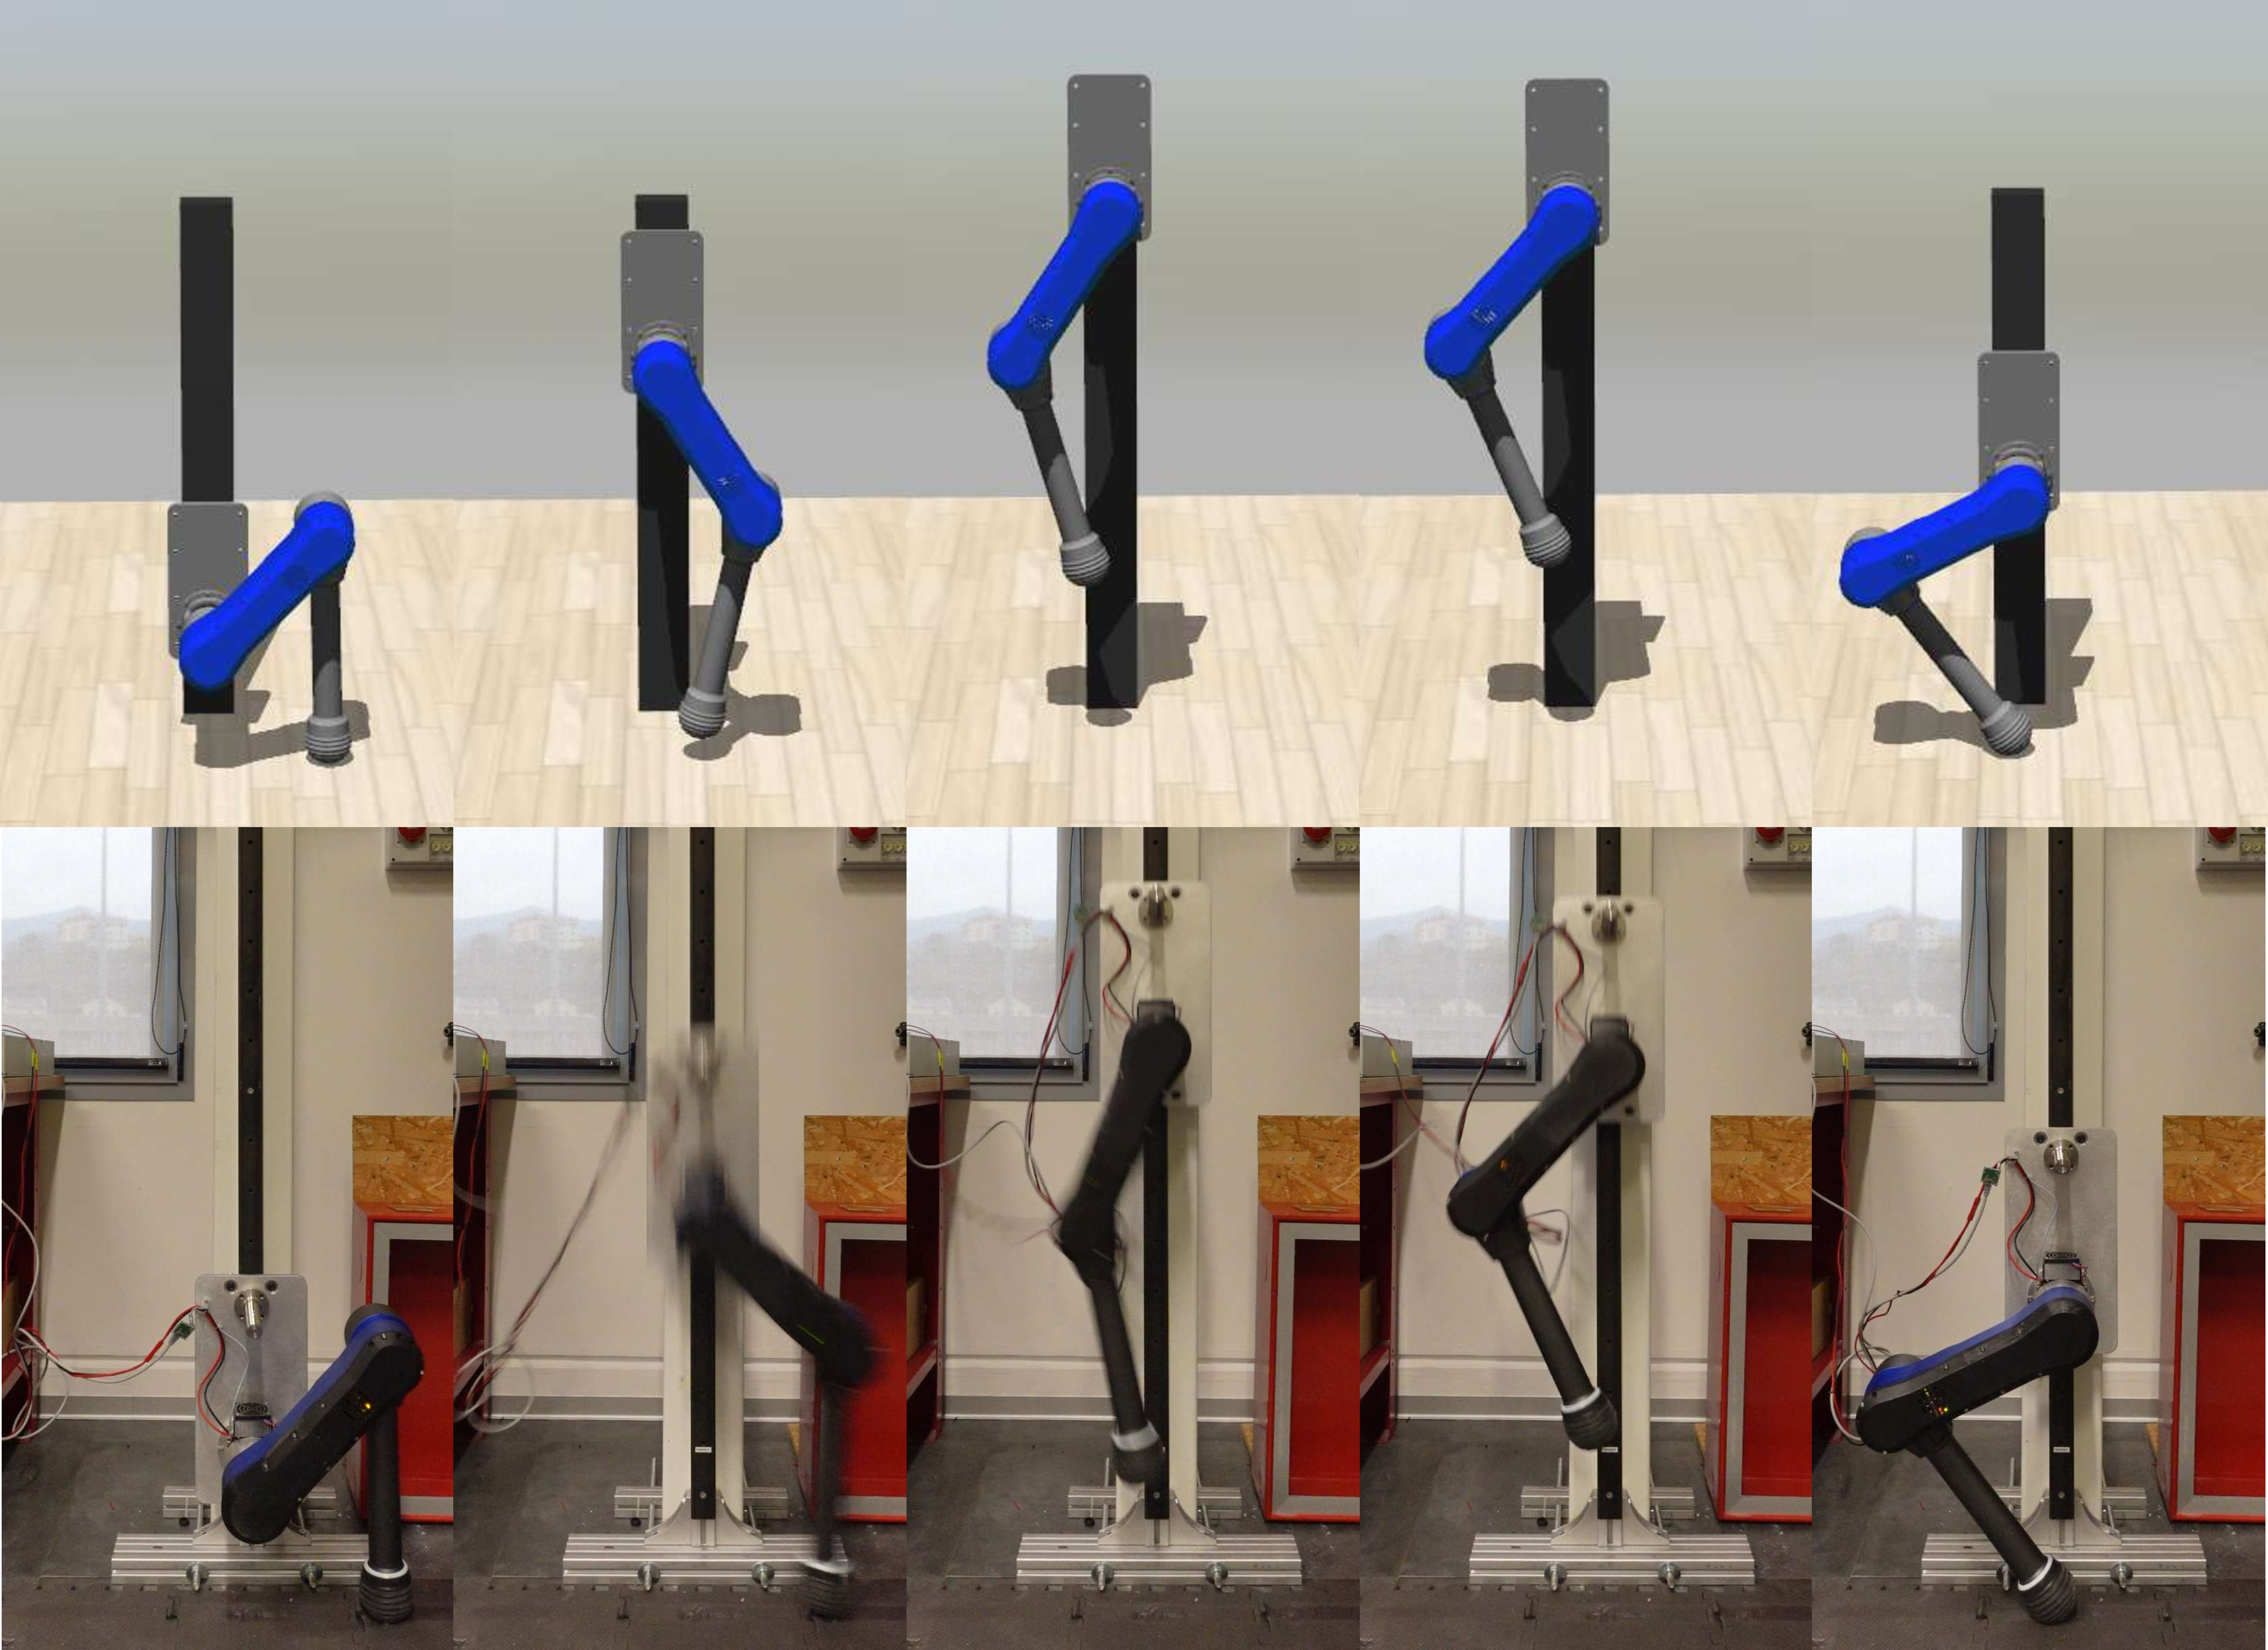
\includegraphics[width=0.98\columnwidth]{images/jumping_sequence_real_sim_compressed.pdf}
    \caption{Snapshots of our quadruped leg prototype performing the optimized jump and landing maneuver obtained with our two-stage TO formulation, in simulation (top) and on the real hardware (bottom), from left to right.}
    \label{fig:jumping_sequence}
\end{figure}

Motivated by the end goal of developing a new electrically powered agile quadruped, we present an in-depth case study revolving around our heavy-duty torque-controllable $12~\mathrm{kg}$ quadruped leg prototype (shown in Fig.~\ref{fig:jumping_sequence}). We choose to focus our attention on the most meaningful and complex task achievable with a single leg setup: the jump. 
% The complexity in performing agile maneuvers increases considerably with the weight of the robot and poses several challenges, both from a mechanical and electrical point of view. 
% links, joints, actuators, power and control electronics are all pushed to their limits. 
\begin{figure*}[t]
    \centering
    \vspace{0.1cm}
    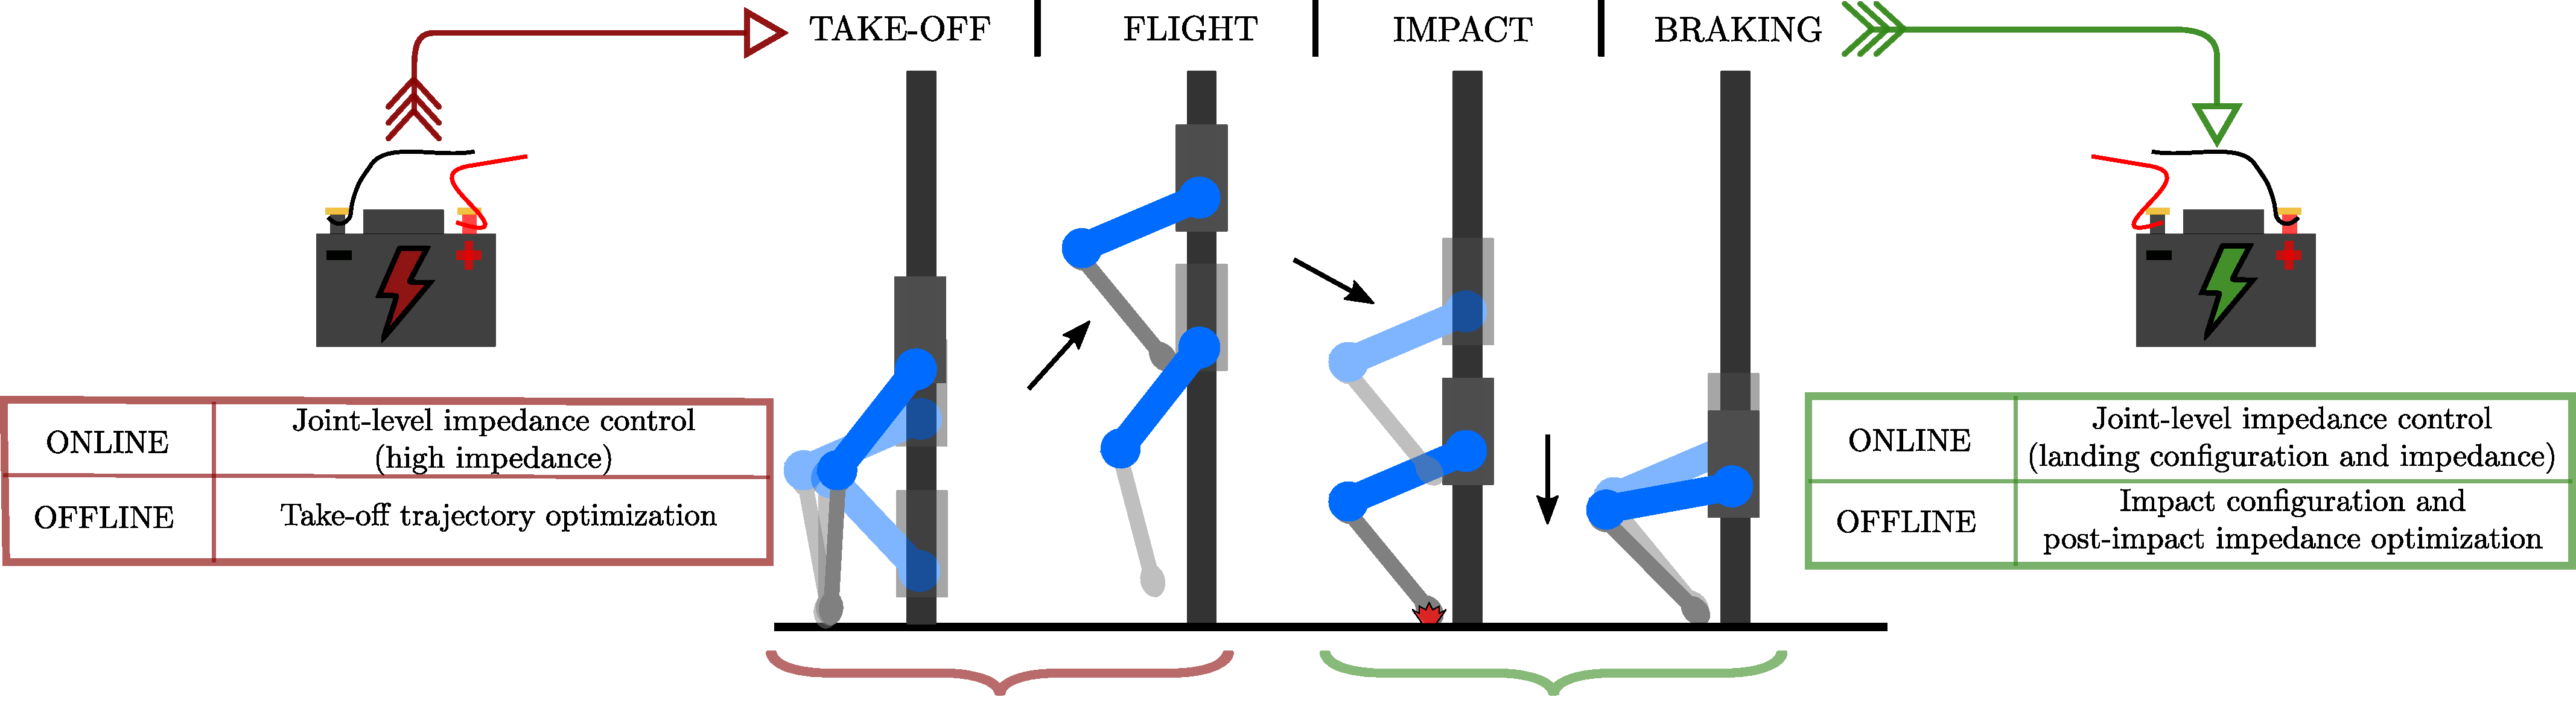
\includegraphics[width=0.9\textwidth]{images/jump_phases_and_pipeline.pdf}
    \caption{A jump sequence decomposed into four main phases, which are synthetically depicted at the center of the figure: the takeoff, the flight, the impact and the braking. During the takeoff phase, energy flows from the power source towards the actuators; after the impact, however, the leg brakes and some of the residual kinetic energy is sent back to the power source and is thus available for regeneration. 
    % Our optimization and control pipeline seeks to exploit these characteristics and, in particular, is made of an offline layer, which houses two separate TO problems, and an online layer, occupied by a simple joint-level impedance controller. 
    }
	\vspace{-0.4cm}
    \label{fig:pipeline}
\end{figure*}
To be able to perform a jumping task while fully exploiting the capabilities of our prototype, we developed a two-stage pipeline (shown in Fig.~\ref{fig:pipeline}) based on Trajectory Optimization (TO), which in recent years has become one of the most successful methods in generating complex motions for robotic systems\cite{agile_bots::nguyen2019optimized,agile_bots::chignoli2021humanoid, agile_bots::roscia2023orientation}.
% \cite{agile_bots::neunert2017trajectory,agile_bots::winkler2018gait,agile_bots::chignoli2021online,agile_bots::nguyen2019optimized,agile_bots::chignoli2021humanoid, agile_bots::roscia2023orientation,agile_bots::carius2019trajectory}.

The core contribution of this work is the development of a two-stage TO pipeline for designing and executing jumping maneuvers, while maximizing energy regeneration and impact mitigation, incorporating also accurate actuation and power flow models.
%    The development of a pipeline made of two sequential TOs for the design and execution of jumping maneuvers, incorporating accurate actuation and power flow models, as well as the maximization of energy regeneration and impact mitigation.
%    The first TO handles the thrust phase and generates a feasible take-off trajectory, while accounting for several hardware contraints.  The second TO problem tackles the impact and post-impact breaking phases and employs suitable energy flow and impact dynamics models, which allow us to maximize the energy regenerated by the actuators during braking, while also minimizing the dissipation of kinetic energy due to the impact with the ground.
 In literature, there exists several works reasoning about impact mitigation and energy recuperation, e.g.~\cite{agile_bots::katz2019mini,agile_bots::hawkes2022engineered,agile_bots::chignoli2021humanoid}. However, to the authors' best knowledge, this is the first time the relationship between ground impact and energy regeneration is explored and accounted for \textit{explicitly} in the context of jump maneuver design for dq0-based field-oriented-controlled robotic systems. The validation of our two TOs and models was performed through extensive trials in simulation and on the real hardware.

The rest of the paper is organized as follows. Section~\ref{sec:prb_def} 
%expands upon the peculiarities of jumping maneuvers and
lays down the premises for our approach and TOs. Section~\ref{sec:formulation} details the formulation of our models and optimization problems, focusing on some pivotal aspects specific to the task under analysis, i.e. the jump. Section~\ref{sec:exp_results} shows the results of our study providing experimental validation for the TO formulations. Finally, Section~\ref{sec:conclusions} sums up and comments on the main results of our case study and highlights possible lines of future research.  
